\documentclass[12pt,a4paper,ngerman]{article}
\usepackage{ifpdf}
\usepackage[utf8x]{inputenc}
\usepackage[ngerman]{babel}
\usepackage{fancyhdr}
\usepackage[pdftex]{graphicx}
\usepackage{graphicx}
\usepackage{amsfonts}
\usepackage{wrapfig}
\usepackage{boxedminipage}
\usepackage{color}
\usepackage{cancel}
\usepackage{subfigure}
\usepackage{url}
\usepackage[numbers]{natbib}

\usepackage{listings}
\definecolor{gray}{rgb}{0.4,0.4,0.4}
\definecolor{darkblue}{rgb}{0.0,0.0,0.6}
\definecolor{cyan}{rgb}{0.0,0.6,0.6}


\lstdefinelanguage{puppet}{
basicstyle=\ttfamily\scriptsize,
keywords={class,package,user,service,present,running,Package,class,include},
%otherkeywords={=>},
morestring=[b]",
morestring=[b]',
stringstyle=\color{black},
identifierstyle=\color{darkblue},
keywordstyle=\color{cyan},
}
\lstdefinelanguage{sh}
{
basicstyle=\ttfamily\scriptsize,
morekeywords={vagrant,su,sudo,puppet,cat,export},deletekeywords={vagrant-puppet}
morestring=[b]",
morestring={[s]{/tmp}{pp}},
keywordstyle=\color{cyan},
}
\lstdefinelanguage{vagrant}
{
basicstyle=\ttfamily\scriptsize,
morestring=[b]",
morekeywords={end,do,config.vm.forward_port},
otherkeywords={config.vm.forward_port,config.vm.provision,puppet.manifests_path,puppet.module_path,puppet.manifest_file},
keywordstyle=\color{cyan},
identifierstyle=\color{darkblue},
stringstyle=\color{black},
morecomment=[l][\color{black}]{\#}
}

\lstdefinelanguage{tree}
{
morekeywords={puppet,manifests,modules,apache,files,templates,my_module},
deletekeywords={apache.pp},
keywordstyle=\color{cyan},
identifierstyle=\color{darkblue},
basicstyle=\ttfamily\scriptsize,
columns=fixed,
}

\lstset{ %
numbers=left,                   % where to put the line-numbers
numberstyle=\scriptsize,      % the size of the fonts that are used for the line-numbers
stepnumber=1,                   % the step between two line-numbers. If it's 1 each line will be numbered
numbersep=5pt,                  % how far the line-numbers are from the code
backgroundcolor=\color{white},  % choose the background color. You must add \usepackage{color}
showspaces=false,               % show spaces adding particular underscores
showstringspaces=false,         % underline spaces within strings
showtabs=false,                 % show tabs within strings adding particular underscores
%extendedchars=false,
frame=single,			% adds a frame around the code
tabsize=2,			% sets default tabsize to 2 spaces
captionpos=b,			% sets the caption-position to bottom
breaklines=true,		% sets automatic line breaking
breakatwhitespace=false,	% sets if automatic breaks should only happen at whitespace
escapeinside={\%*}{*)}          % if you want to add a comment within your code
}

\usepackage[top=2.5cm, bottom=2cm, left=2.5cm, right=2.5cm]{geometry} 

\clubpenalty = 10000
\widowpenalty = 10000 \displaywidowpenalty = 10000

\makeatletter
\fancypagestyle {plain}{
  \lhead {}
  \rhead {\@title}
  \cfoot {}
  \lfoot {\copyright 2012, Anders Malmborg und Michael Haslgrübler}
  \rfoot {\thepage}
  \renewcommand {\footrulewidth }{1pt}
}
\makeatother

%\textwidth17cm
%\textheight24.5cm  
%\textwidth24.5cm
%\textheight17cm  
\headheight15pt

\usepackage{hyperref}
\hypersetup{
    bookmarks=false,         % show bookmarks bar?
    unicode=true,          % non-Latin characters in Acrobat’s bookmarks
    pdftoolbar=false,        % show Acrobat’s toolbar?
    pdfmenubar=false,        % show Acrobat’s menu?
    pdffitwindow=false,     % window fit to page when opened
    pdfstartview={FitW},    % fits the width of the page to the window
    pdftitle={Deliver with Puppet},    % title
    pdfauthor={Anders Malmborg und Michael Haslgr\"ubler},     % author
    pdfsubject={Deliver with Puppet},   % subject of the document
    %pdfcreator={Creator},   % creator of the document
    %pdfproducer={Producer}, % producer of the document
    pdfkeywords={Vagrant} {Puppet} {Continous Delivery}, % list of keywords
    pdfnewwindow=true,      % links in new window
    colorlinks=false,       % false: boxed links; true: colored links
    linkcolor=red,          % color of internal links
    citecolor=green,        % color of links to bibliography
    filecolor=magenta,      % color of file links
    urlcolor=cyan           % color of external links
}

%\makeatletter
%\ifpdf
%\pdfinfo {
%	/Author (\@author)
%	/Title (\@title)
%	/Subject ()
%	/Keywords ()
%}
%\fi
%\makeatother

\title{Deliver with Puppet}
\author{Anders Malmborg and Michael Haslgruebler}

\newcommand{\reffig}[1]{, siehe Abbildung~\ref{#1}}
\newcommand{\reflst}[1]{, siehe Listing~\ref{#1}}
%\newcommand{\graphicsext}{eps}
\newcommand{\graphicsext}{png}



\begin{document}
 \begin{titlepage}
     \begin{flushright}{\huge Continous Delivery with Puppet}
	\end{flushright}
	\hrule
      
      \begin{flushright}
	  {\large Anders Malmborg und Michael Haslgrübler}\\
	  \today
	\end{flushright}
 \end{titlepage}

\pagestyle{plain}

\section{Einleitung}

\subsection{Ausgangssituation}
%TODO: erster absatz extrem abgehackt
Iteratives Vorgehen bei der Entwicklung von Applikationen ist mittlerweile sehr verbreitet. Jede Iteration erweitert meist die Applikation mit neuer Funktionalität. Jede Implementierung und Konfiguration einer neuen Funktionalität sollte außerdem in der Iterationsphase qualitätsgesichert werden. Zusätzlich zu UnitTests, welche einzelne Teile prüfen, sind Integrationstests mit einer laufenden Applikation zwingend erforderlich - sei es automatisch oder manuell.

Jede Applikation beinhaltet außerdem Konfigurationen, im banalsten Fall sind das Einstellungen für den Zugriff auf eine Datenbank oder Schalter welche Teilfunktionalitäten aktivieren. Je nach den Konfigurationsmöglichkeiten können mehrere Installationen notwendig sein um die korrekte Funktionsweise einer Applikation, in all ihren Variationen, sicherzustellen.

Für die Source-Code-Übersetzung, Testausführung und Paketiereung der Applikation helfen Continous Integration Systeme wie \cite{jenkins}. Aber wie automatisiert man den nächste Schritt - die automatische Installation und Konfiguration von mehreren Servern? 

Für diese Problemstellung haben wir uns nach einer Lösung umgesehen und mit Puppet einen gangbaren Weg gefunden. 

\cite{puppet} oder auch \cite{chef} sind so genannte Configuration Management(CM) Lösungen. Zusammengefasst bietet ein CM-Lösung die Möglichkeit den erwarteten Zustand eines Systems (hier Server) zu beschrieben und bei Abweichungen Mechanismen um das System in dem erwarteten Zustand zu versetzt.

Folgende Probleme wollten wir adressieren und dafür Lösungen finden:
\begin{itemize}
\item Automatische Installation und Konfiguration nach erfolgreichen Build im Jenkins.
\begin{itemize}
\item trotz Paketierung in Web Archivs (WARs) waren einige Konfigurationen, wie Datenbank-Parametern, manuell einzutragen.
\end{itemize}
\item Zentrale Definition, welche Applikationen mit welcher Konfiguration wo, auf welchen Servern, zu laufen haben.
\item Neue virtuelle Servers sollten einfach von einem Basis-Image aufgesetzt werden und mit Puppet fertig konfiguriert werden, inklusive beispielsweise Apache und Tomcat.
\item Gleiche Mechanismen und selbes Vorgehen bei der Test-/QA- und Produktionsumgebung.
\end{itemize}

In der Entwicklung heißt das in erster Linie Softwarecode der commited wird, der gebaut werden kann und die automatisierten Tests besteht soll auch installiert werden. Damit können wir gewährleisten bzw. überprüfen das die Software zu jedem Zeitpunkt einsatzbereit ist und nicht nur auf einem Entwicklungs-PC funktioniert.

\subsection{Puppet Einführung}

Puppet benutzt eine Domain-Specific-Language(DSL) um den Zustand eines System zu beschreiben. Der Code wird strukturiert in Manifeste und Module.

\begin{wrapfigure}{r}{8cm}
\vspace{-20pt}
\begin{boxedminipage}{8cm}
Für die Entwicklung von Puppet Module und Manifeste bietet sich \cite{geppeto} an. Geppeto bringt Code Completion und Syntax Highlighting mit und kommt als Standaloneapplikation oder als Plugin für eine bestehende Eclipse-Installation. 
\end{boxedminipage}
\vspace{-20pt}
\end{wrapfigure}

Ein Manifest ist ein Puppet "Program". Module sind für die Puppet-EntwicklerIn ähnlich wie Libraries für Programmierer. Ein Großteil der Manifeste und Module machen die Definition von Ressourcen aus. Eine Ressource ist ein atomarer Typ eines Systems, es entspricht einer physisches Identität eines Computersystems. Ein Beispiel für eine solche Ressource, wäre ein Benutzer oder eine Datei. In Listing \ref{puppet-add-user} wird die Ressource user \lstinline$puppetdemo$ und dazugehörige Ressource file \lstinline$/home/puppetdemo$ definiert. Der Aufruf \lstinline$sudo puppet apply manifest/user.pp$ führt es aus und muss mit 'sudo' aufgerufen werden damit Verzeichnis und Benutzer angelegt werden können, da dies nur der Administrator darf.
Mit \lstinline$puppet resource user puppetdemo$ wird die Informationen zum neu angelegten Benutzer ausgegeben\reflst{puppet-add-user-info}.


\begin{lstlisting}[language=sh,caption=User mit Puppet anlegen, label=puppet-add-user]
$ cat manifest/user.pp 
node default {
    user {
        'puppetdemo' :
            ensure => present,
            home => '/home/puppetdemo',
            shell => '/bin/bash',
    }
    file {
        '/home/puppetdemo' :
        ensure => 'directory',
        owner => 'puppetdemo',
        group => 'puppetdemo',
    }
}
$ sudo puppet apply manifest/user.pp 
notice: /Stage[main]//Node[default]/User[puppetdemo]/ensure: created
notice: /Stage[main]//Node[default]/File[/home/puppetdemo]/ensure: created
notice: Finished catalog run in 0.36 seconds
\end{lstlisting}
\begin{lstlisting}[language=puppet,caption=Anzeige der Benutzerinformation in Puppet, label=puppet-add-user-info]
user { 'puppetdemo':
  ensure => present,
  gid    => '1004',
  home   => '/home/puppetdemo',
  shell  => '/bin/bash',
  uid    => '1002',
}
\end{lstlisting}

Eine Aufzählung der vom Puppet unterstützen Ressourcen wird mit \lstinline$puppet resource --types$ ausgegeben. Die Ressourcen sind im Core Types Cheat Sheet \url{http://docs.puppetlabs.com/puppet_core_types_cheatsheet.pdf} auch gut beschrieben.

%Im Beispiel\reffig{puppet-user}, sehen wir wie wir einen Benutzer und eine Datei mit der Puppet DSL anlegen.

%\begin{figure}
%  \begin{center}
%    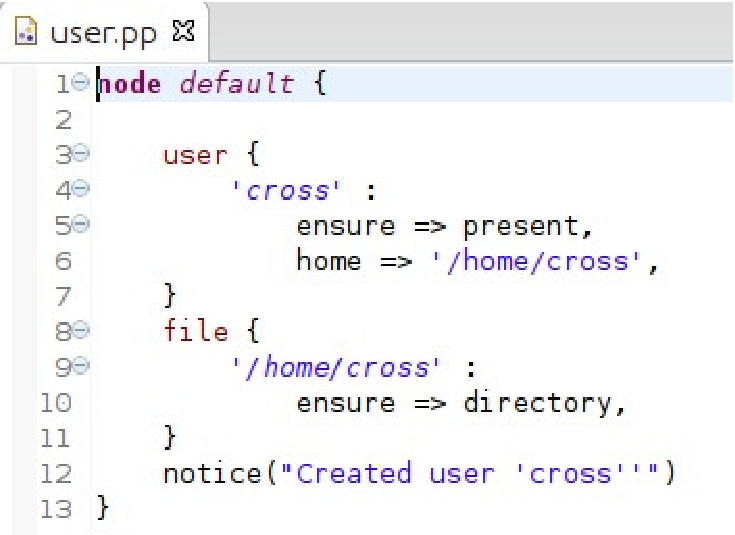
\includegraphics[width=0.7\textwidth]{images/user.pdf}
%  \end{center}
%  \caption{User mit Puppet anlegen}
%  \label{puppet-user}
%\end{figure}


%Der Manifest user.pp legen wir in einem Verzeichnis manifests ab\reffig{puppet-manifestdir}.

%\begin{figure}
%  \begin{center}
%    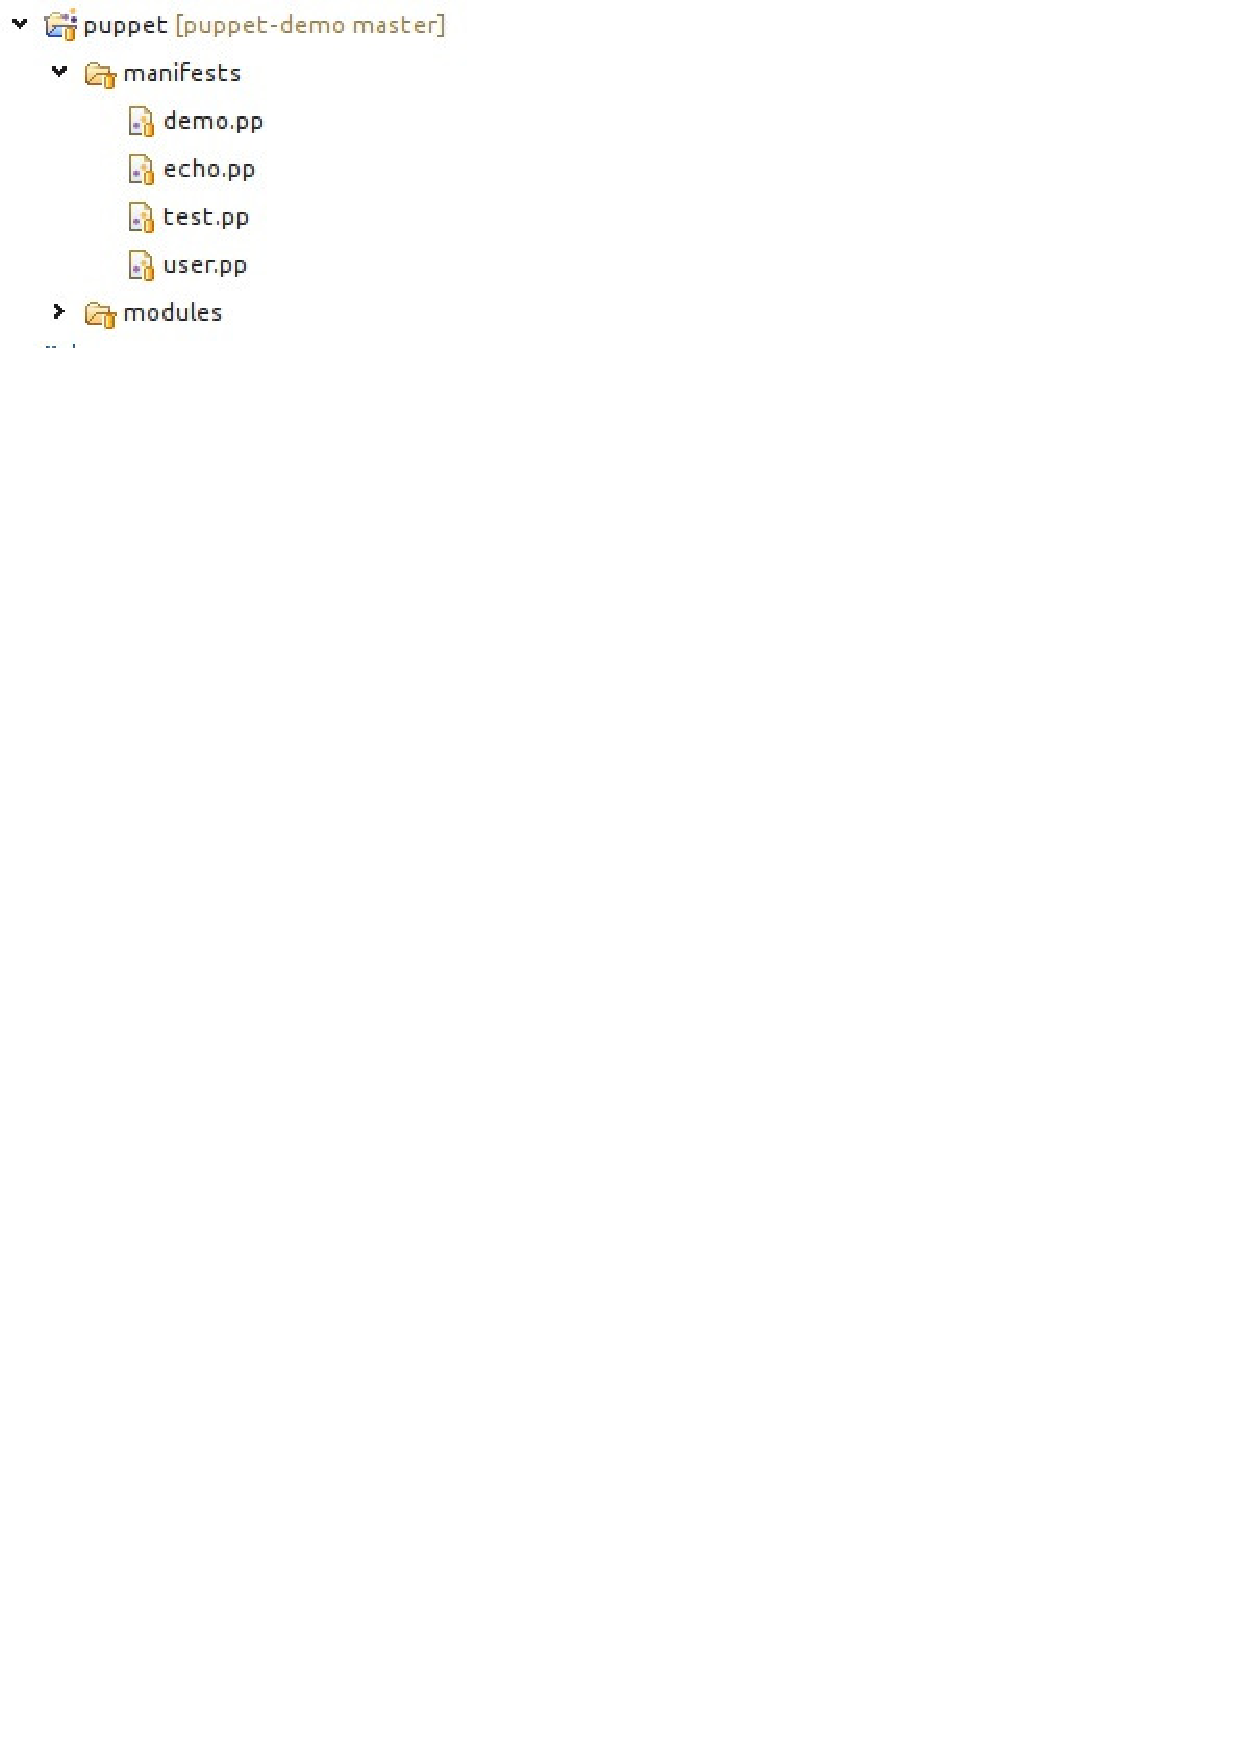
\includegraphics[width=0.7\textwidth]{images/manifestdir.pdf}
%  \end{center}
%  \caption{Puppet Manifest Verzeichnis}
%  \label{puppet-manifestdir}
%\end{figure}


\subsection{Testbox mit Vagrant}
Zum kennenlernen vom Puppet stellt Puppet Labs eine virtuelle Maschine für VMware beziehungsweise VirtualBox zur Verfügung unter \url{http://info.puppetlabs.com/download-learning-puppet-VM.html}. 

Für die Entwicklung und Tests von Puppet Modulen und Manifeste empfehlen wir \cite{vagrant}. Vagrant ist eine Konfigurationstool für die Verwaltung von virtuellen Maschinen mit VirtualBox. Es kann in weiterer Folge auch Puppet, Chef oder Shell Scripts benutzen kann um die virtuelle Maschine zu konfigurieren. Vagrant benützt virtuelle Maschine die in so genannte Boxen gepackt sind. Zusätzlich zu der virtuellen Maschine beinhaltet eine Box unter anderem Chef and Puppet. Die Boxen sind portabel - sie laufen auf alle Platformen wo Vagrant laufen. Mit Vagrant ist es relativ einfach die Puppet Module und Manifeste auf unterschiedliche Zielumgebungen zu verifizieren indem man sie auf unterschiedliche Boxen testet. Vagrant via Paketmanager für Linux installiert werden oder von den entsprechenden Downloadseiten heruntergeladen werden.

%TODO: erklären warum wir vagrant verwenden

\begin{wrapfigure}{l}{5cm}
\vspace{-15pt}
\begin{boxedminipage}{5cm}
Eine Liste mit vorgefertigten Vagrant Boxen gibt es übrigens auf \url{http://www.vagrantbox.es/}
\end{boxedminipage}
\vspace{-15pt}
\end{wrapfigure}

Nachdem Vagrant und VirtualBox installiert worden sind, können wir eine Box zum Testen aufsetzen. In unserem Fall verwenden wir eine 64 Bit Version von Debian Squeeze. Diese beinhaltet eine Minimalinstallation mit den für Vagrant üblichen Vorbereitungen: SSH Key Setup, VirtualBox Guest Additions, Puppet und Ruby, siehe auch \url{http://vagrantup.com/v1/docs/base_boxes.html}.

\begin{lstlisting}[language=sh,caption=Download der Vagrant Box, label=vagrant-add]
vagrant box add debian_squeeze_64 http://dl.dropbox.com/u/937870/VMs/squeeze64.box
\end{lstlisting}

\begin{wrapfigure}{r}{4.5cm}
\vspace{-20pt}
\begin{boxedminipage}{4.5cm}
 Die Vagrant Boxen werden unter Unix in \lstinline!$HOME/.vagrant.d/boxes! installiert. 
Falls man dies ändern will kann man die Umgebungsvariable \lstinline$VAGRANT_HOME$ setzen:
\begin{lstlisting}[language=sh,label=vagrant-home,frame=none,numbers=none]
export VAGRANT_HOME=$HOME/vagrant_home
\end{lstlisting}
\end{boxedminipage}
\vspace{-20pt}
\end{wrapfigure}
 

Nachdem dem Download steht uns jetzt die  Vagrant Box \lstinline$debian_squeeze_64$ zur Verfügung. Nun können wir in ein beliebiges Verzeichnis wechseln und eine initiale Konfiguration basierend auf der Box anlegen\reflst{vagrant-init}.

\begin{lstlisting}[language=sh,caption=Vagrant initialisieren, label=vagrant-init]
vagrant init debian_squeeze_64
\end{lstlisting}

Diese initiale Konfiguration beinhaltet alles was Vagrant zum Konfigurieren und Starten der Maschine braucht, es sind keine weiteren Einstellungen mehr nötig und wir können diese starten\reflst{vagrant-up}.

\begin{lstlisting}[language=sh,caption=Starten der Vagrant Maschine, label=vagrant-up]
vagrant up
\end{lstlisting}

Nachdem die virtuelle Maschine gestartet worden ist, können wir mit ssh einsteigen\reflst{vagrant-ssh}. Unter Windows ist dieser Befehl derzeit nicht verfügbar und man muss deshalb mit Tools wie \cite{putty} darauf zugreifen.
\begin{lstlisting}[language=sh,caption=Mit ssh in der Vagrant Maschine einsteigen, label=vagrant-ssh]
vagrant ssh
\end{lstlisting}
 
Zum Aktivieren von Puppet müssen wir unseren \lstinline$Vagrantfile$ bearbeiten. Dieser liegt im Verzeichnis wo wir den Befehl \lstinline$vagrant init$ ausgeführt haben. Diese Datei beinhaltet bereits Einträge für Puppet, welche jedoch auskommentiert sind. Nach dem entfernen der Kommentarzeichen für die Sektion \lstinline$config.vm.provision :puppet$, tragen wir unter \lstinline$puppet.manifests_path$ und \lstinline$puppet.module_path$ ein wo unsere Manifeste und Module liegen. Als \lstinline$puppet.manifest_file$ tragen wir \lstinline$user.pp$ ein. Zum Testen von einer späteren Apache-Installation wird Port 6400 im Host auf Port 80 im Guest weitergeleitet:\lstinline$config.vm.forward_port 80, 6400$. Das ganze sollte dann in etwa wie in Listing \ref{vagrantprovisioning} aussehen.
  
\begin{lstlisting}[language=vagrant,caption=Puppet Provisioning in Vagrantfile konfigurieren, label=vagrantprovisioning]
  config.vm.forward_port 80, 6400  
  config.vm.provision :puppet do |puppet|
    puppet.manifests_path = "~/git/puppet-demo/puppet/manifests"
    puppet.module_path = "~/git/puppet-demo/puppet/modules"
    puppet.manifest_file  = "user.pp"
  end
\end{lstlisting} 

Bei dieser Änderung müssen wir die Vagrantbox neu laden, da geteilte Verzeichnisse nur beim Starten des Hosts erkannt und automatisch gemounted werden. Zusätzlich dazu wird beim Starten das Provisioning, durch Puppet mit den Anweisungen aus \lstinline$user.pp$ durchgeführt. Mit \lstinline$puppet ssh$ steigen wir und verifizieren dass der User 'puppetdemo' mit Home-Verzeichnis /home/puppetdemo vorhanden ist\reflst{vagrant-reload}.

\begin{lstlisting}[language=sh,caption=Vagrant Box neu laden, label=vagrant-reload]
vagrant reload
notice: /Stage[main]//Node[default]/User[puppetdemo]/ensure: created
notice: /Stage[main]//Node[default]/File[/home/puppetdemo]/ensure: created
notice: Finished catalog run in 0.35 seconds

$ vagrant ssh
Welcome to your Vagrant-built virtual machine.

$ sudo su - puppetdemo
puppetdemo@precise32:~$ pwd
/home/puppetdemo
\end{lstlisting}

Mit \lstinline$vagrant provisioning$ kann das Puppet Manifest erneut ausgeführt werden. Ohne Änderungen im Manifest oder in der virtuellen Maschine passiert nichts. Würde der Benutzer \lstinline$puppetdemo$ zum Beispiel entfernt, wird er wieder beim nächsten Provision-Vorgang wieder angelegt.
Will man das Puppet Manifest in der virtuellen Maschine manuell ausführen, ist der \lstinline$puppet.manifests_path$ als \lstinline$/tmp/vagrant-puppet/manifest$ gemounted\reflst{vagrant-apply}.

\begin{lstlisting}[language=sh,caption=Puppet apply im Box, label=vagrant-apply]
$ sudo puppet apply /tmp/vagrant-puppet/manifests/user.pp
No LSB modules are available.
notice: Finished catalog run in 0.04 seconds
$ sudo deluser puppetdemo
Removing user `puppetdemo' ...
Warning: group `puppetdemo' has no more members.
Done.
$ sudo puppet apply /tmp/vagrant-puppet/manifests/user.pp
No LSB modules are available.
notice: /Stage[main]//Node[default]/User[puppetdemo]/ensure: created
notice: Finished catalog run in 0.39 seconds
\end{lstlisting}

Vagrant kann wie VirtualBox die Maschine stilllegen mit \lstinline$vagrant suspend$ bzw mit \lstinline$vagrant resume$ wieder fortsetzen. Zum Starten und Stoppen kann man \lstinline$vagrant up$ bzw mit \lstinline$vagrant halt$ verwenden.  Sollte man die Box nicht mehr benötigen kann Sie mit \lstinline$vagrant destroy$ unwiderruflich löschen. Das Vagrantfile bleibt jedoch erhalten, somit kann man wieder bei Null anfangen und mit \lstinline$vagrant up$ die Box inklusive Provisioning mit Puppet wieder aufsetzen.

\section{Apache Webserver und eine Applikation mit HTML und JavaScript mit Puppet installieren}
Nachdem wir die Grundlagen von Puppet und Vagrant jetzt kurz kennengelernt haben, installieren wir einen Apache Webserver. Da es wahrscheinlich ist, dass Apache für andere Applikationen auch genutzt wird, wird der Puppet Code dafür in einem Module abgelegt. Module sind wiederverwendbare Einheiten vom Code und Daten. Die Struktur eines Modules ist auf \url{http://docs.puppetlabs.com/learning/modules1.html} beschrieben, wie auszugsweise in Abbildung \ref{module_structure} dargestellt.
% Puppet Module Cheat Sheet \url{docs.puppetlabs.com/module_cheat_sheet.pdf}
\begin{lstlisting}[language=tree,caption=Puppet Module Struktur, label=module_structure]
my_module
|-- files
|   `-- my_file.txt
|-- manifests
|   `-- init.pp
`-- templates
    `-- my_template.erb
\end{lstlisting}


Auf die gleiche Ebene wie das manifests-Verzeichnis legen wir das Verzeichnis \lstinline$modules$ an, darunter die Datei \lstinline$apache/manifests/init.pp$ und entsprechenden Verzeichnisse\reflst{apache-module}.
%use to generate this tree --noreport -n puppet
\begin{lstlisting}[language=tree,caption=Verzeichnisstruktur für den apache-Module, label=apache-module]
puppet
|-- manifests
|   `-- user.pp
`-- modules
    `-- apache
        `-- manifests
            `-- init.pp
\end{lstlisting}

Die Datei \lstinline$modules/apache/manifests/init.pp$ ist recht kompakt und zeigt auf einen Blick einen der großen Vorteile von Puppet. Die Ressourcen \lstinline$package$ und \lstinline$service$ verstecken die Komplexität und die plattformspezifische Vorgänge für Installation von Paketen und das Starten der Dienste\reflst{apache-init.pp}.
\begin{lstlisting}[language=puppet,caption=Inhalt von modules/apache/manifests/init.pp, label=apache-init.pp]
class apache {
        package {
                'apache2' :
                        ensure => present,
        }
        service {
                'apache2' :
                        ensure => running,
                        require => Package["apache2"]
        }
}
\end{lstlisting}

Um ein Modul in einem Manifest verwenden zu können, reicht es lediglich \lstinline$include apache$\reflst{setupapache.pp} zu schreiben.
\begin{lstlisting}[language=puppet,caption=Inhalt von manifests/setupapache.pp, label=setupapache.pp]
include apache
\end{lstlisting}

In Vagrantfile ändern wir jetzt die Zeile \lstinline$puppet.manifest_file  = "user.pp"$ auf \lstinline$puppet.manifest_file  = "setupapache.pp"$ und geben auf der Kommandozeile \lstinline$vagrant provision$ ein\reflst{provisioning_apache}.

\begin{lstlisting}[language=sh,caption=vagrant provisioning für Apache, label=provisioning_apache]
$ vagrant provision
[default] Running provisioner: Vagrant::Provisioners::Puppet...
[default] Running Puppet with /tmp/vagrant-puppet/manifests/setupapache.pp...
notice: /Stage[main]/Apache/Package[apache2]/ensure: ensure changed 'purged' to 'present'
notice: Finished catalog run in 97.25 seconds
\end{lstlisting}

Wenn wir auf unseren Browser die lokale Adresse über, den weitergeleiteten, Port 6400 aufrufen, können wir feststellen dass der Apache Webserver läuft\reffig{apache}.
\begin{figure}
  \begin{center}
    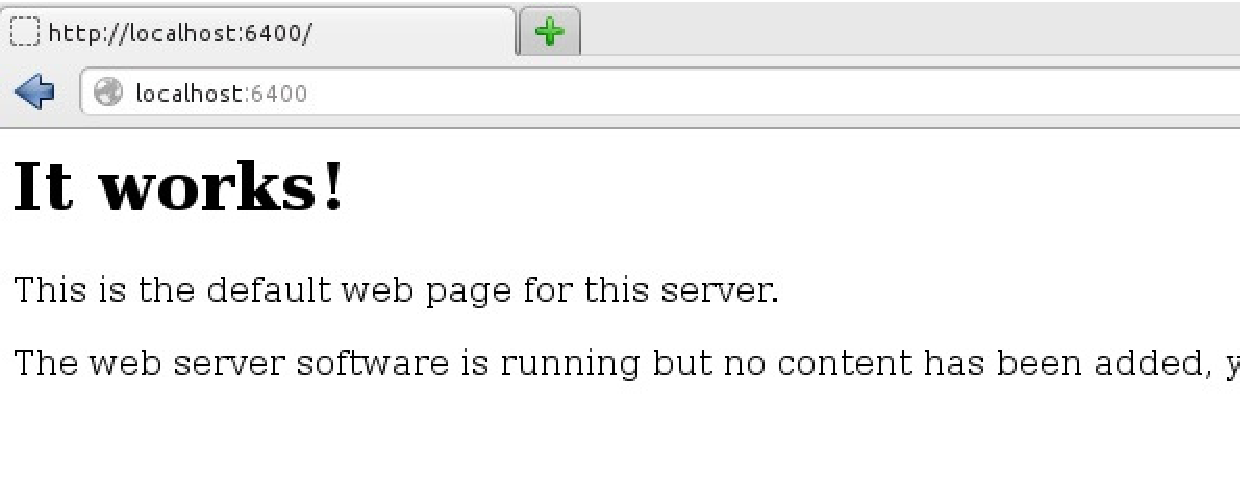
\includegraphics[width=0.4\textwidth]{images/apache.pdf}
  \end{center}
  \caption{Apache aufrufen}
  \label{apache}
\end{figure}

Als nächstes lassen wir Puppet die Dateien für die Applikation in das Apache Wurzel Verzeichnis (\lstinline$/var/www/$) kopieren. Folgender Eintrag in Vagrantfile stellt das Host-Verzeichnis \lstinline$~/git/puppet-demo/puppet-demoapp/src/main/webapp$ als Guest-Verzeichnis \lstinline$/demoapp$ zur Verfügung\reflst{vagrantsharedfolder}. Das Guest-Verzeichnis dient als Quelle für die Kopie.
\begin{lstlisting}[language=vagrant,caption=Shared folders in Vagrantfile konfigurieren, label=vagrantsharedfolder]
config.vm.share_folder "demoapp", "/home/vagrant/demoapp", "~/git/puppet-demo/puppet-demoapp/src/main/webapp"
\end{lstlisting}

Mit dem Manifest \lstinline$manifests/demoapp.pp$ für die Installation der Applikation\reflst{puppetdemoapp}, definieren wir das Puppet die Dateien vom zuvor spezifizierten Verzeichnis \lstinline$/demoapp$ nach \lstinline$/var/www/$ kopieren sollen, das Ganze ist im Module demoapp gekapselt\reffig{puppet-demo-module}.
\begin{lstlisting}[language=puppet,caption=Puppet Manifest für die Applikation, label=puppetdemoapp]
include apache
include demoapp
\end{lstlisting}

\begin{lstlisting}[language=puppet,caption=Puppet Module demoapp,label=puppet-demo-module]
class demoapp($demoappname='demoapp') {
    file {
        "/var/www/$demoappname" :
        ensure => directory,
        source => '/home/vagrant/demoapp',
        require => Package['apache2'],
        recurse => true,
    }
}
\end{lstlisting}


Durch die Änderung der geteilten Verzeichnisse im Vagrantfile ist es notwendig die Vagrant Box neu zu starten um die Änderung aktiv werden zu lassen:  \lstinline$vagrant reload$\reflst{reloaddemoapp}.
\begin{lstlisting}[language=sh,caption=Puppet reload mit Provisioning der Applikation, label=reloaddemoapp]
$ vagrant reload
[default] Attempting graceful shutdown of VM...
[default] Clearing any previously set forwarded ports...
[default] Forwarding ports...
[default] -- 22 => 2222 (adapter 1)
[default] -- 80 => 6400 (adapter 1)
[default] Creating shared folders metadata...
[default] Clearing any previously set network interfaces...
[default] Booting VM...
[default] Waiting for VM to boot. This can take a few minutes.
[default] VM booted and ready for use!
[default] Mounting shared folders...
[default] -- demoapp: /demoapp
[default] -- v-root: /vagrant
[default] -- v-pp-m0: /tmp/vagrant-puppet/modules-0
[default] -- manifests: /tmp/vagrant-puppet/manifests
[default] Running provisioner: Vagrant::Provisioners::Puppet...
[default] Running Puppet with /tmp/vagrant-puppet/manifests/demoapp.pp...
notice: /Stage[main]//File[/var/www/demoapp]/ensure: created
...
notice: /File[/var/www/demoapp/index.html]/ensure: defined content as '{md5}90a8d419b9c7b43b09ba73abebaf8f4c'
...
notice: Finished catalog run in 1.34 seconds
\end{lstlisting}

Nach Abschluss des Neustarts erfolgt auch automatisch wieder der Provisioning Vorgang durch Puppet und wir können unsere neue Webapplikation über den Browser aufrufen\reffig{demoapp}.
\begin{figure}
  \begin{center}
    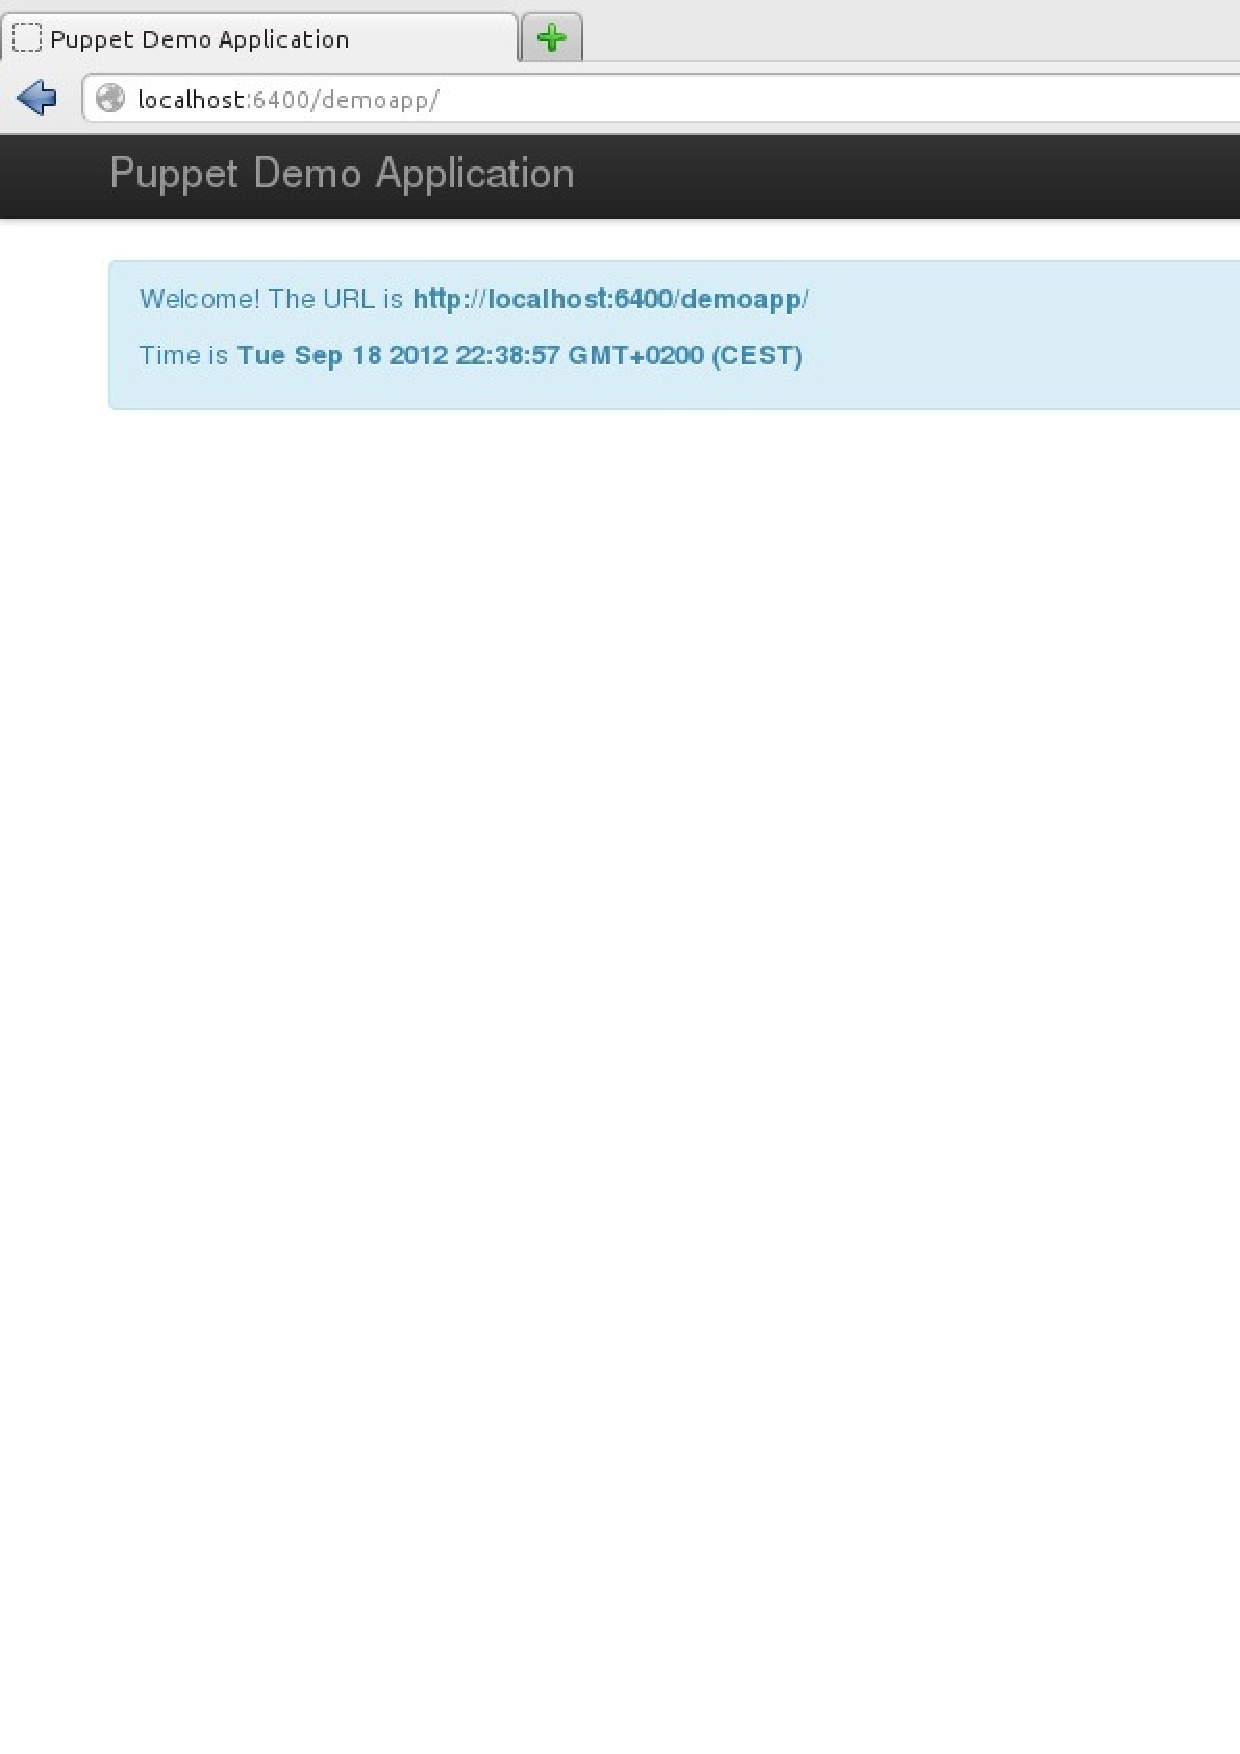
\includegraphics[width=0.4\textwidth]{images/demoapp.pdf}
  \end{center}
  \caption{Die Applikation im Browser}
  \label{demoapp}
\end{figure}

Eine Änderung in der Datei \lstinline$index.html$ wird bei Puppet im Provisioning-Vorgang (\lstinline$vagrant provision$) erkannt und Puppet aktualisiert die Datei auch in \lstinline$/var/www/$\reflst{provisionapp}.
\begin{lstlisting}[language=sh,caption=Puppet Provisioning nach Änderung von index.html, label=provisionapp]
$ vagrant provision
[default] Running provisioner: Vagrant::Provisioners::Puppet...
[default] Running Puppet with /tmp/vagrant-puppet/manifests/demoapp.pp...

notice: /File[/var/www/demoapp/index.html]/content: content changed '{md5}90a8d419b9c7b43b09ba73abebaf8f4c' to '{md5}0a4ee5bb63c3e5c29cc54cf36a4be23c'

notice: Finished catalog run in 0.71 seconds
\end{lstlisting}

\section{Puppet am Server}

Nachdem dem erfolgreichen erstellen erster Manifeste, geht es nun darum wie man die Manifeste auf einem Server verlagert und eine ganze Serverfarm damit betreibt. Grundsätzlich unterscheiden wir bei Puppet zwischen zwei Typen Puppet Master und Puppet Agent. Der Puppet Agent ist auf einem x-belieben Server installiert und kontaktiert eine zentrale Einheit, den Puppet Master, um von ihn gesteuert zu werden. 

\subsection{Puppet Server-Agent-Workflow}

Der Puppet Server-Agent-Workflow funktioniert grundsätzlich nach dem Pull Prinzip, d.h. der Puppet Agent fragt aktiv beim Puppet Master nach was zu tun ist, er fordert einem \textit{Catalog} an in dem er dem Master seinem Namen und seine Informationen über sich selbst, sogenannte \textit{facts} mitteilt. Ein \textit{fact} wäre zum Beispiel das Betriebssystem des Agent. Der Puppet Master identifiziert und sucht nach Arbeitsanweisungen für den Agent. Der Master compiliert aus allen anwendbaren Manifesten einen \textit{Catalog} und sendet ihn zurück an den Agent. Dieser wendet den \textit{Catalog} an d.h. es wird versucht den durch den \textit{Catalog} definierten Zustand herzustellen. Das Herstellen dieses Zustandes wird protokolliert und dann an den Puppet Master gesendet. Dieser Report kann zu einem späteren Zeitpunkt ausgewertet werden.

%TODO: make picture

\subsection{Arbeitsanweisungen für den Agent suchen}

Wenn der Puppet Master vom Puppet Agent kontaktiert wird, wird er mithilfe seines Hostnamen identifiziert und der Puppet Master liest das Manifest \lstinline$/etc/puppet/manifests/site.pp$ ein und sucht nach einer passenden \lstinline$node$ Definition. Wenn der Master nun vom server1.example.org kontaktiert wird wird dieser die Ausgabe \lstinline$hello server1!$ erzeugen, analog für server2. Statt alle Server einzeln zu definieren kann man auch das Schlüsselword default verwenden damit werden die beinhaltende Anweisungen auf allen Servern die den Master kontaktieren ausgeführt werden. 

%TODO: was passiert bei kontakt von server 3

\begin{lstlisting}[language=puppet,caption=Node Definitionen in /etc/puppet/manifests/site.pp, label=puppet-node-classifier]
node server1.example.org {
    notice("hello server1!)
}

node server2.example.org {
    include apache
    notice("hello server2!)
}

node default {
    notice("hello server")
}

\end{lstlisting}  

\subsection{Alternative: External Node Classifier}
     
\begin{lstlisting}[caption=External Node Classifier Konfiguration des Puppet Master, label=puppet-enc-config]
[master]
  node_terminus = exec
  external_nodes = /usr/local/bin/my_node_classifier
\end{lstlisting} 

Alternativ zu obigen deklarativen Ansatz kann Puppet zusätzlich auch einen External Node Classifier verwenden.  Ein External Node Classifier ist ein Script dem als Argument der Puppet Agent Name übergeben wird und der eine \lstinline$YAML$ Datei ausgibt. Die YAML Datei enthält eine Liste von Klassen und Parametern welche dem Knoten zugewiesen werden.  

Im vorigen Beispiel hat die Knotendeklaration\reflst{puppet-node-classifier} für den server2 das \lstinline$apache$ Modul enthalten, analog dazu müsste der ENC das YAML Dokument\reflst{puppet-enc-yaml-param}, ohne die letzte Zeile zurückliefern.  

Interessant wird das Ganze erst wenn der ENC mit einem Konfigurationswerkzeug gekoppelt wird, in dem dynamisch Konfigurationen erstellt werden können. Ein solches Werkzeug wäre das \cite{puppetdashboard}. Nachteil hierbei ist es, das parametrisierte Klassen derzeit nicht verwaltet werden können. In unserem obigen Beispiel könnten wir die Demoapplikation unter einer anderen URL auch verfügbar machen in dem wir den Klassenparameter demoappname überschreiben\reflst{puppet-enc-yaml-param}.

%TODO: über eigen implementierung schreiben?

\begin{lstlisting}[caption=ENC's YAML mit Klassenparameter , label=puppet-enc-yaml-param]
name: server2.example.org
---
classes: 
    apache:
    demoapp: 
        demoappname: mydemoapp
\end{lstlisting} 

\subsubsection{Dashboard}

Das Puppet Dashboard kann nicht nur als ENC verwendet werden sondern ist primär eigentlich ein Reporting Tool. In Abbildung \ref{dashboard-overview} sieht man eine Übersicht über den aktuellen Knoten. Im oberen Teil sieht man welche Gruppen, Klassen und Parameter dem Knoten zugeordnet sind. In unserem Fall sind das die Klassen \lstinline$apache$ und \lstinline$demoapp$. Die Klassen müssen im Modulpfad (\lstinline$/etc/puppet/modules/$) des Puppet Master liegen. Desweiteren sieht man eine Übersicht über die Änderungen am Knoten, als sich der Puppet Agent mit dem Master verbunden hat und das Provisioning durchgeführt wurde. Der Provisioning-Vorgang wird im Dashboard\reffig{dashboard-detail} und in der Ausgabe des Puppet Agent festgehalten\reffig{puppet-agent-run}.
\begin{figure}[ht]
\centering
\subfigure[Übersicht eines Knoten]{
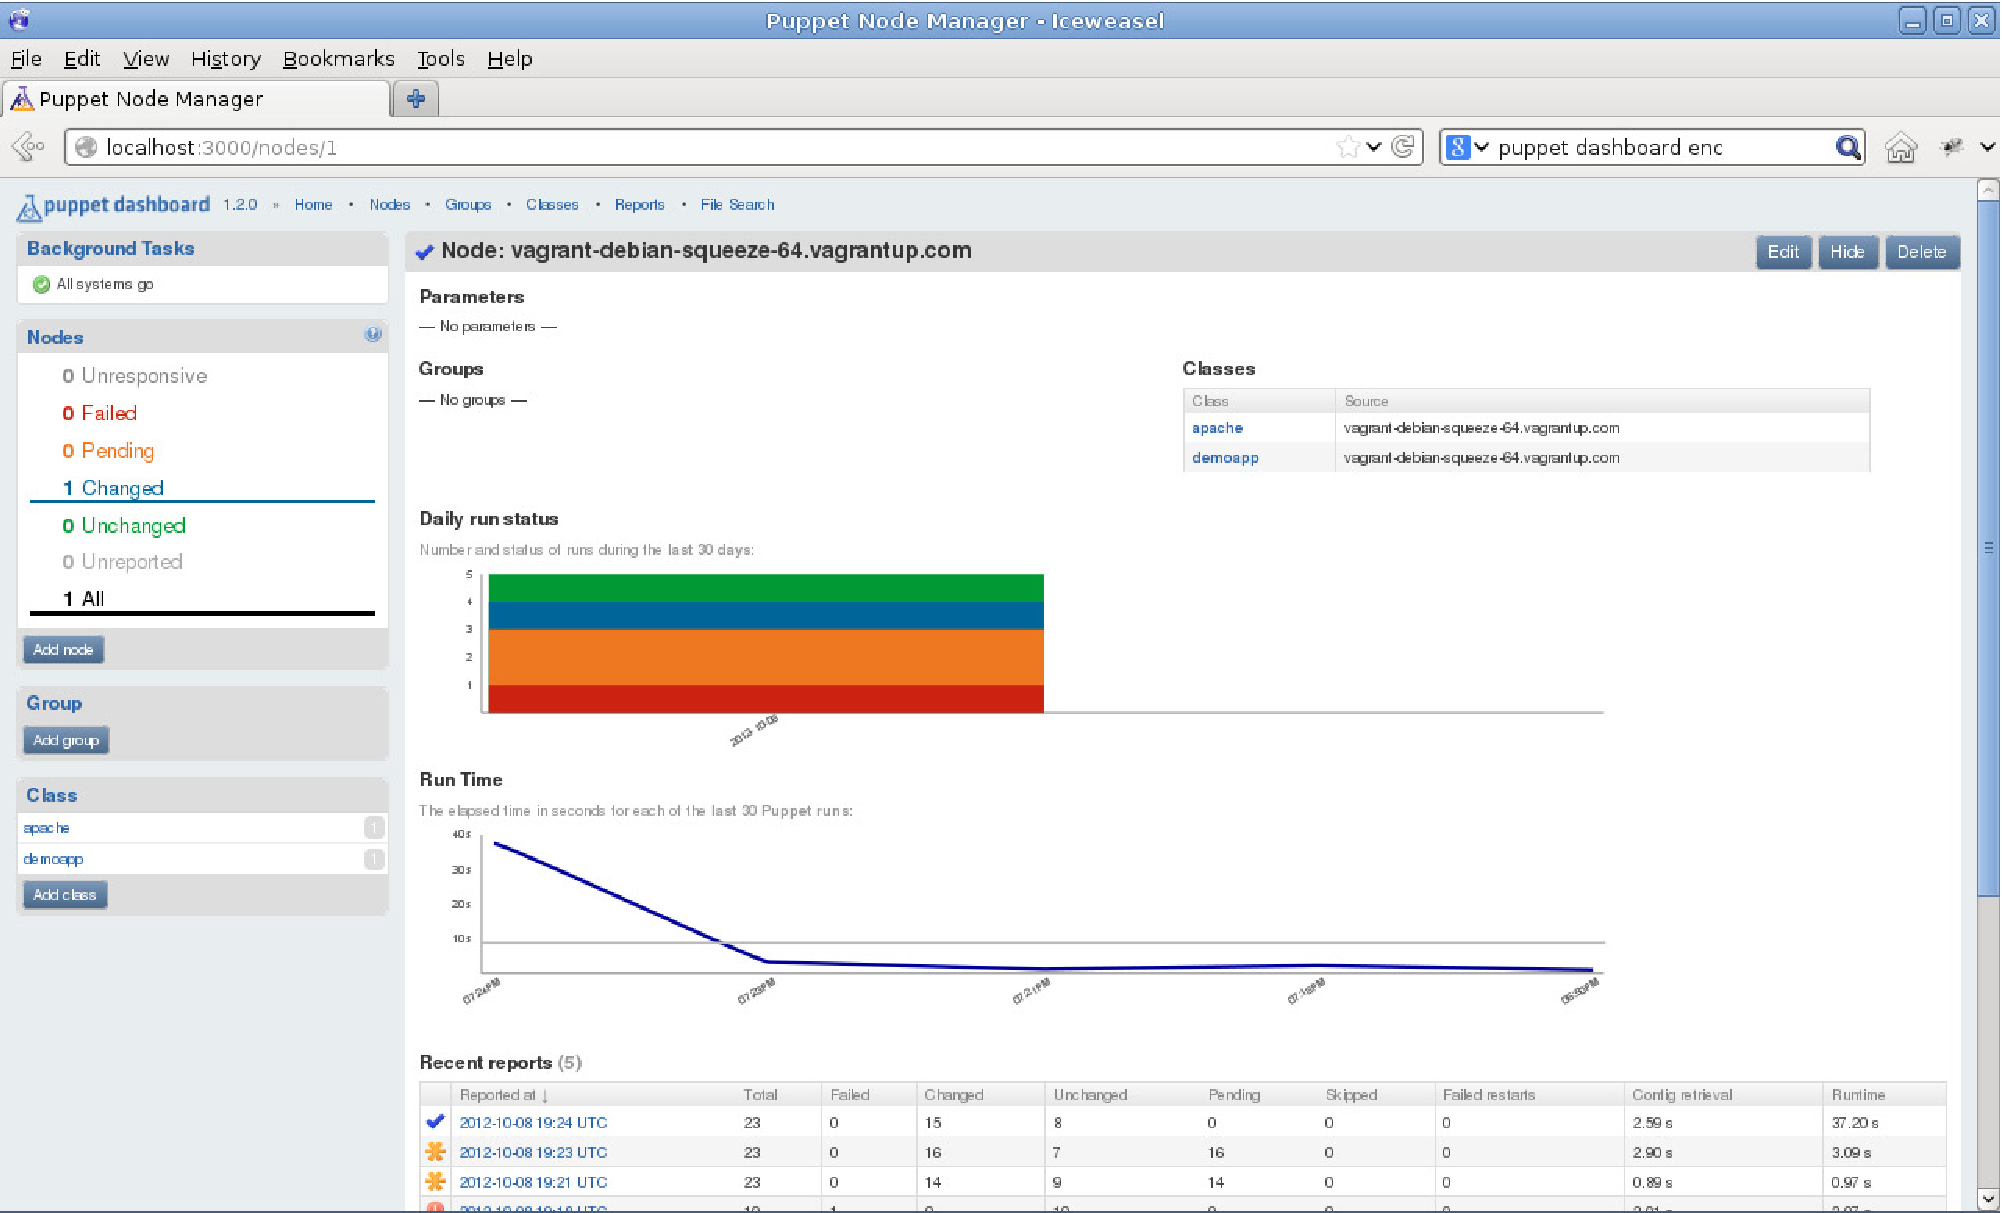
\includegraphics[height=5.2cm]{images/dashboard2.pdf}
	\label{dashboard-overview}
}
\subfigure[Änderungen im Dashboard]{
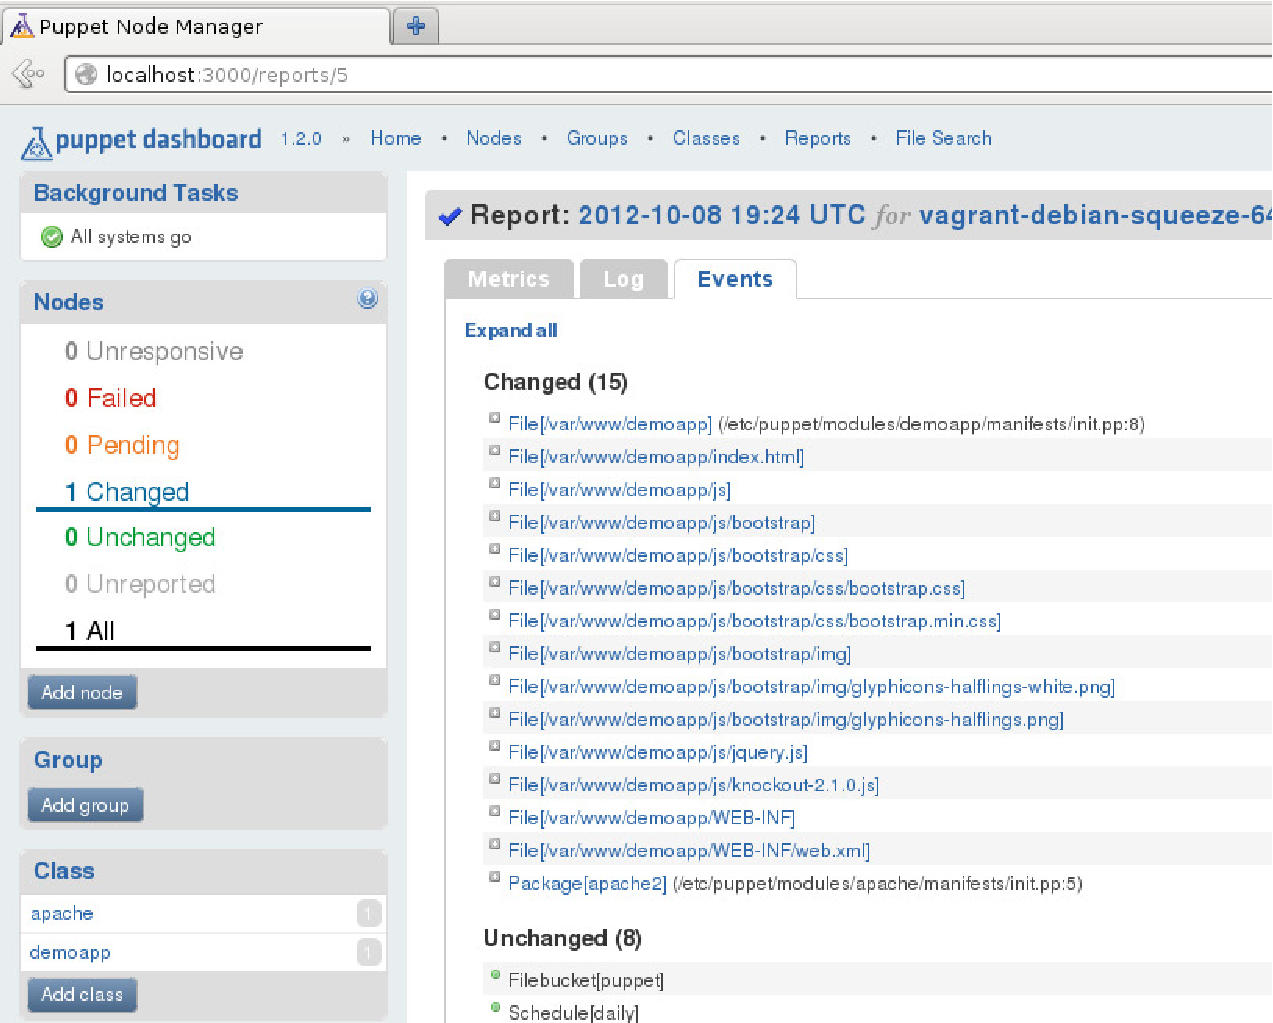
\includegraphics[height=5.2cm]{images/dashboard1.pdf}
	\label{dashboard-detail}
}
\caption{Puppet Dashboard}
\label{dashboard}
\end{figure}

\begin{lstlisting}[language=sh,caption=Puppet Agent Run durchführen , label=puppet-agent-run]
$ puppet agent --test --server vagrant-debian-squeeze-64.vagrantup.com
info: Caching catalog for vagrant-debian-squeeze-64.vagrantup.com
info: Applying configuration version '1349723897'
notice: /Stage[main]/Apache/Package[apache2]/ensure: ensure changed 'purged' to 'present'
notice: /Stage[main]/Demoapp/File[/var/www/demoapp]/ensure: created
...
notice: /File[/var/www/demoapp/js/knockout-2.1.0.js]/ensure: defined content as '{md5}235475c7c3dc43c7cb7f6125be536c32'
notice: Finished catalog run in 35.07 seconds
\end{lstlisting}

\section{Resumeé}

Wir wollten für uns mit Puppet und Vagrant Lösungen für folgende Probleme finden:
\begin{itemize}
\item Automatische Installation und Konfiguration nach erfolgreichen Build im Jenkins 
\item Zentrale Definition, welche Applikationen mit welcher Konfiguration wo, auf welchen Servern, zu laufen haben.
\item Neue virtuelle Servers sollten einfach von einem Basis-Image aufgesetzt werden und mit Puppet fertig konfiguriert werden, inklusive beispielsweise Apache und Tomcat.
\item Gleiche Mechanismen und Vorgehen bei der Test-/QA- und Produktionsumgebung.
\end{itemize}

Beim Jenkins Build wird nicht nur die Software compiliert sondern es erfolgt auch eine Paketierung.  Die Konfiguration kann aber nicht Teil der Paketierung sein sondern muss zu einem späteren Zeitpunkt bestimmt werden. Weiters muss definiert werden, wenn möglich zentral, wo diese Applikationen mit welcher Konfiguration zu laufen haben. Puppet in Verknüpfung mit einem ENC bietet uns genau diese Funktionalität. Wir definieren im ENC, welcher Server mit welcher Software von Puppet ausgestattet werden soll und über Parameter der dazugehörigen Puppet Module definieren wir, wie diese Software konfiguriert wird. 

Mithilfe von Puppet können wir auf Basis eines Standard-Image, wie in obigen bei Vagrant eingesetzt, einen Server fertig konfigurieren und auf unsere Bedürfnisse anpassen und das mit dem selben Mechanismus -- wiederholbar -- in jeder Umgebung, sei es QA oder Produktion.

%TODO: ist das ein gutes resumee?

\section*{Autoren}

\newcommand{\authorboxheight}{5cm}
\begin{minipage}[t][\authorboxheight]{0.45\textwidth}
\textbf{Anders Malmborg}
\vskip0.3cm
\begin{wrapfigure}{l}{0.3\textwidth}
\vspace{-20pt}

\includegraphics[width=0.3\textwidth]{images/anders.jpg}
\vspace{-20pt}
\end{wrapfigure}
hat jahrezehntelange Erfahrung in der Applikations- und Produktentwicklung im C++ und JavaEE Umfeld und arbeitet als IT Freelancer im automotive Bereich. 
\end{minipage}
\hspace{0.1\textwidth}
\begin{minipage}[t][\authorboxheight]{0.45\textwidth}
\textbf{Michael Haslgrübler}
\vskip0.3cm
\begin{wrapfigure}{l}{0.3\textwidth}
\vspace{-20pt}

\includegraphics[width=0.3\textwidth]{images/michael.jpg}
\vspace{-20pt}
\end{wrapfigure}
hat mehrjährige Erfahrung in JavaEE Entwicklungsumfeld in der Automotive und Immobilienbranche. Er administriert seit Jahren einen Linux-Root-Server für diverse Kunden.
\end{minipage}

\bibliographystyle{apalike2}
\bibliography{document}

\end{document}
